\section{Beispiele}

\begin{multicols}{2}
Gib ein Bespiel für eine Strecke an, so dass alle folgenden Aussagen zutreffen:
- die Strecke hat die Ordnung 1
- mit einem P-Regler KR (Gegenkopplung) ergibt sich ein stabiler Regelkreis bei $0 < K_R < 4$
- mit einem P-Regler KR (Gegenkopplung) ergibt sich ein instabiler Regelkreis bei $K_R > 4$
Lösung: a) 1 Pol Ordnung 1, b) Pol in LHE (stabil bei kleinem $K_R$)  c) Wegen Instailtiät bei grossem $K_R$ Nullstelle in RHE, d) Symetrische Lage erlaubt einfacherres Einstellen e) $G_s=\frac{1}{4}\cdot\frac{s-a}{s+a} \quad a \ > \ 0, beliebig$ 
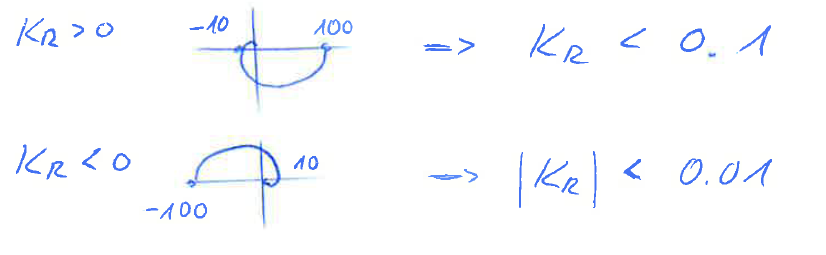
\includegraphics[width=9cm]{./images/beispiele/beispiel17.png}
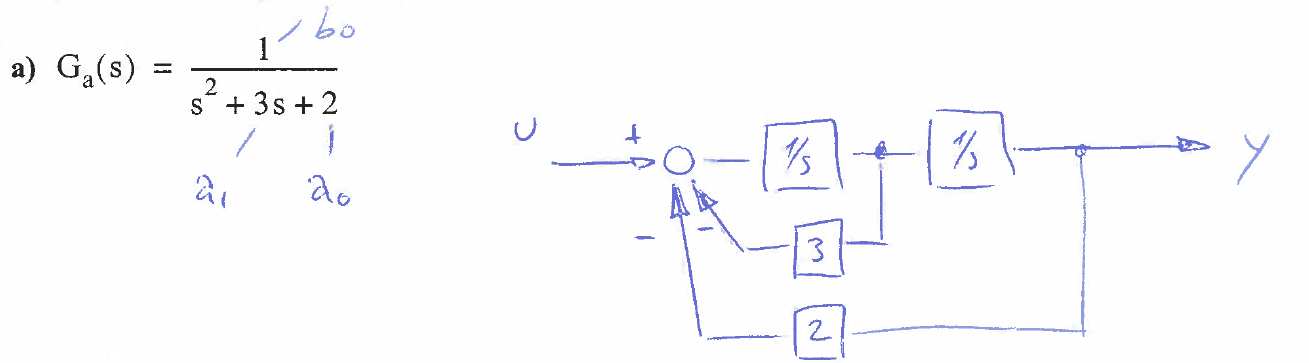
\includegraphics[width=9cm]{./images/beispiele/beispiel1.png}
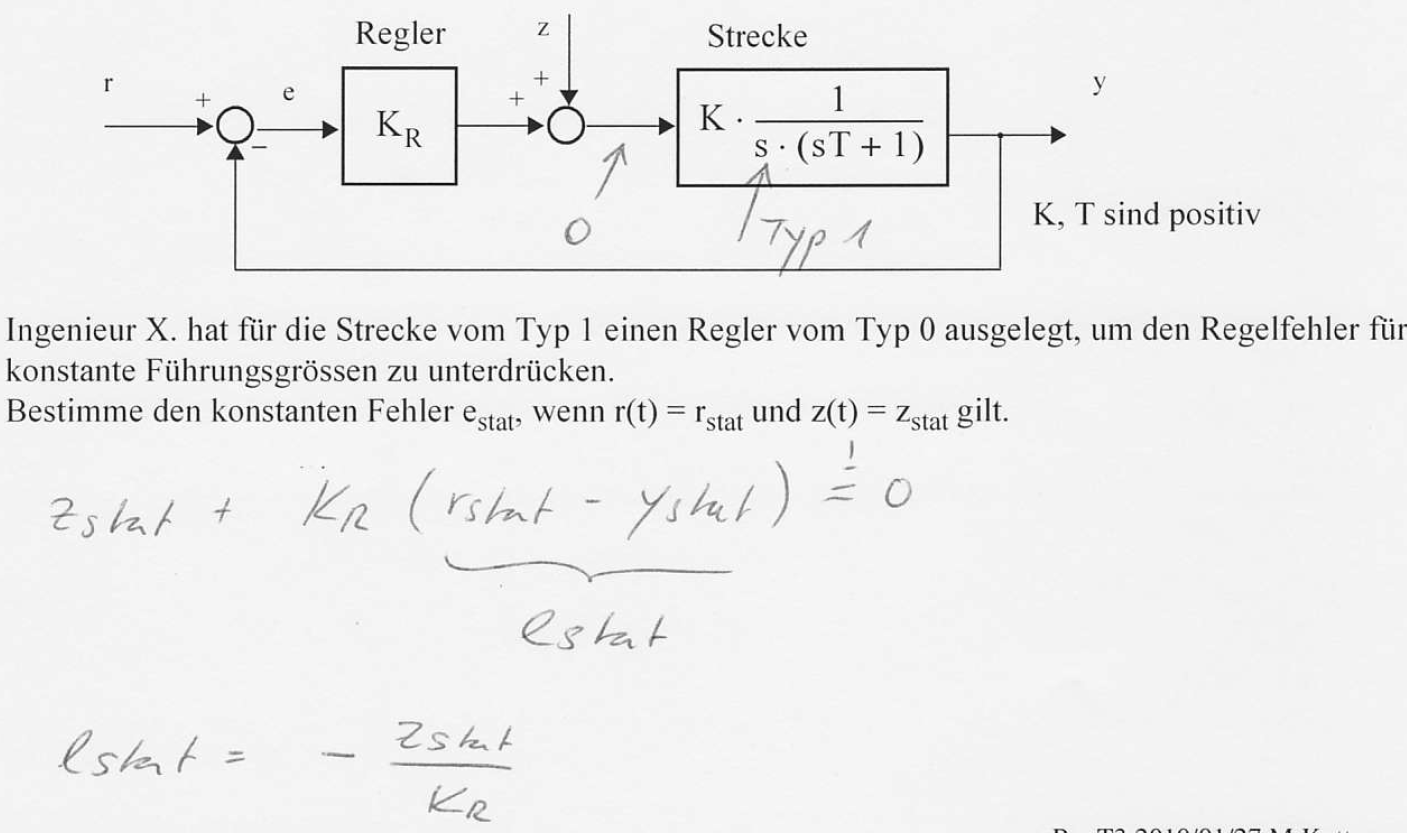
\includegraphics[width=9cm]{./images/beispiele/beispiel2.png}
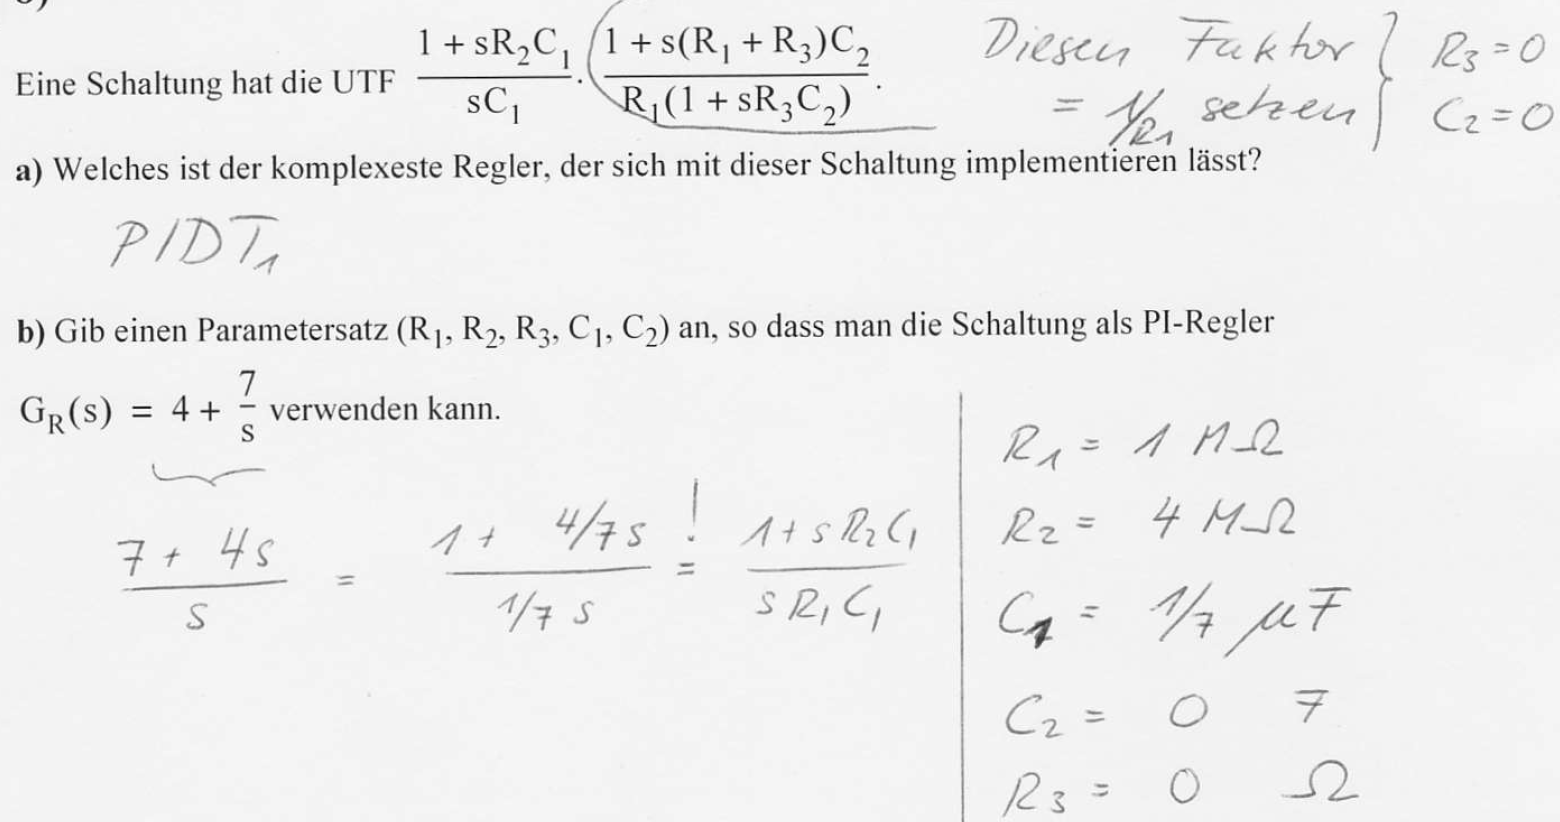
\includegraphics[width=9cm]{./images/beispiele/beispiel3.png}
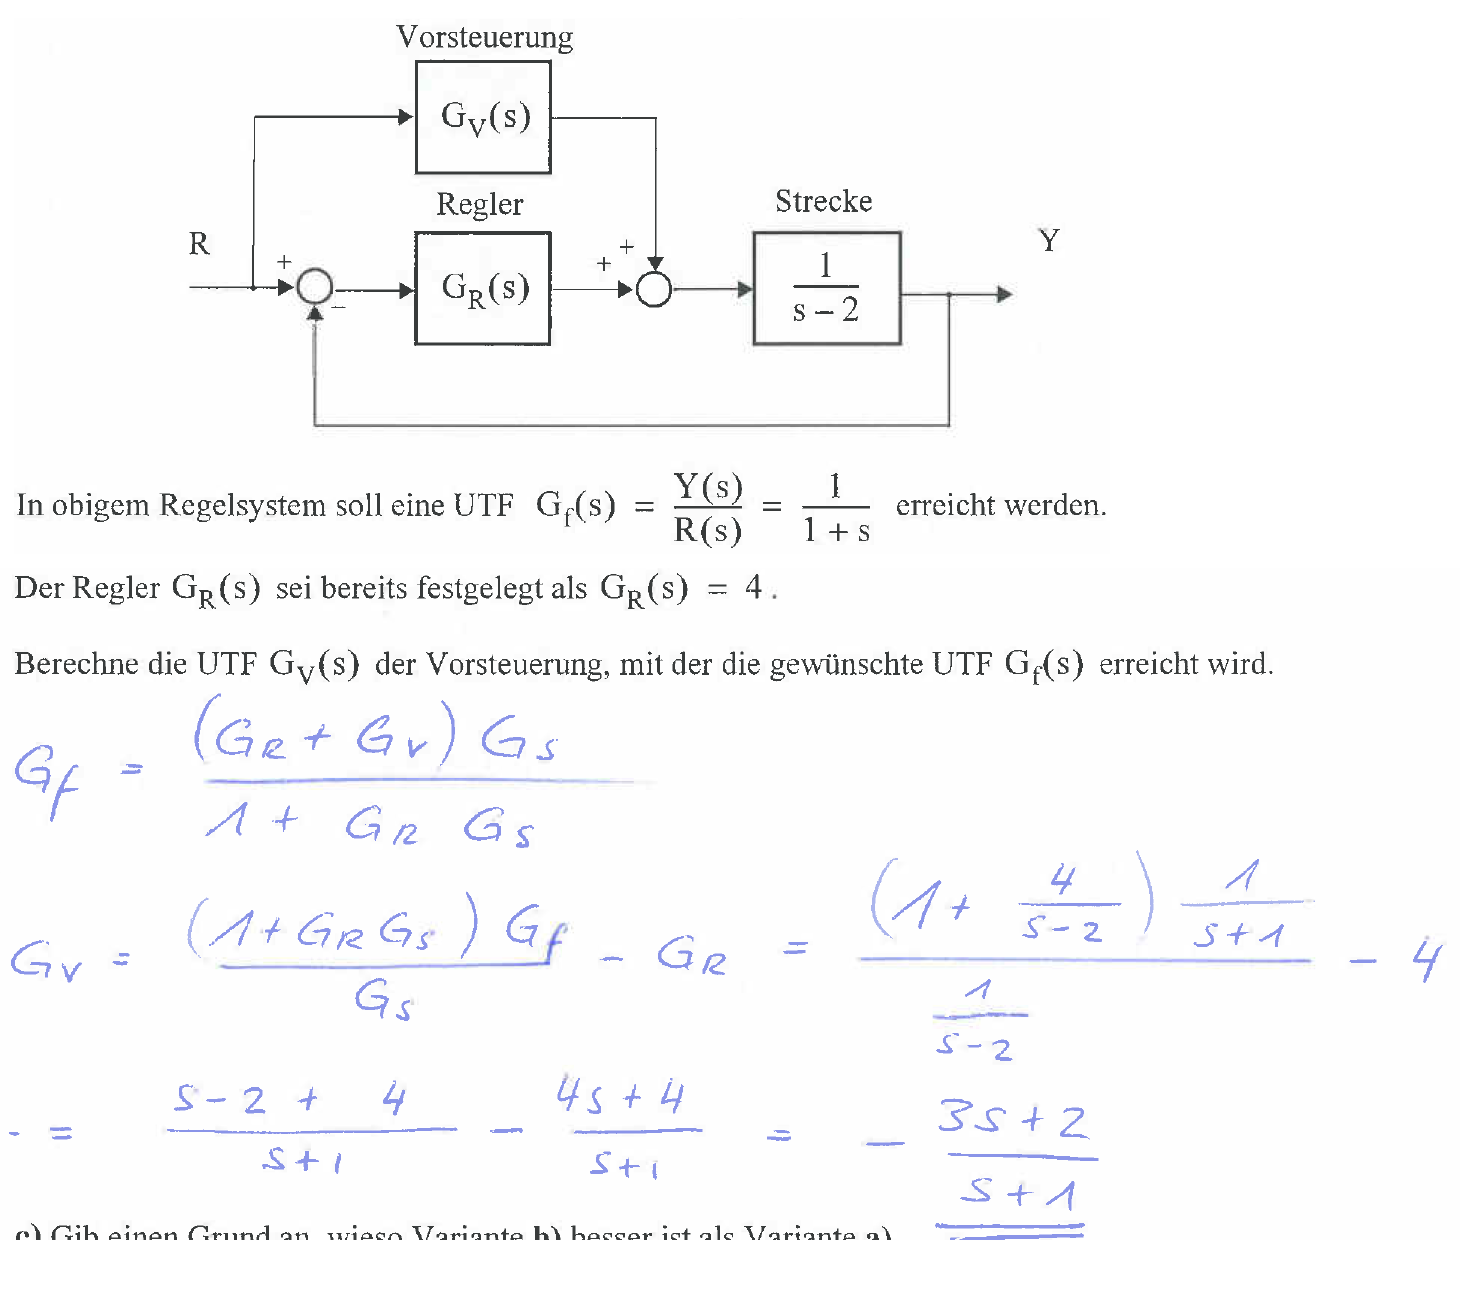
\includegraphics[width=9cm]{./images/beispiele/beispiel4.png}
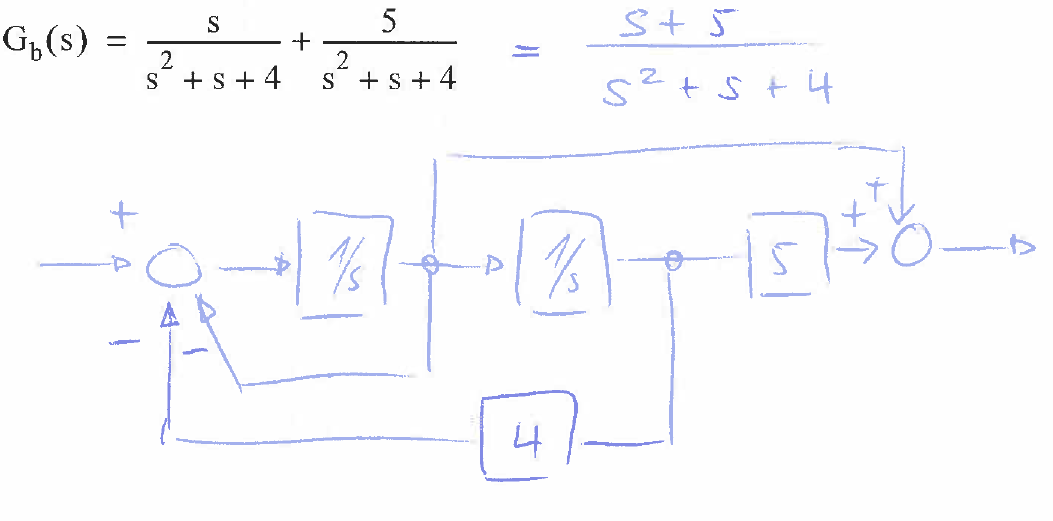
\includegraphics[width=9cm]{./images/beispiele/beispiel5.png}
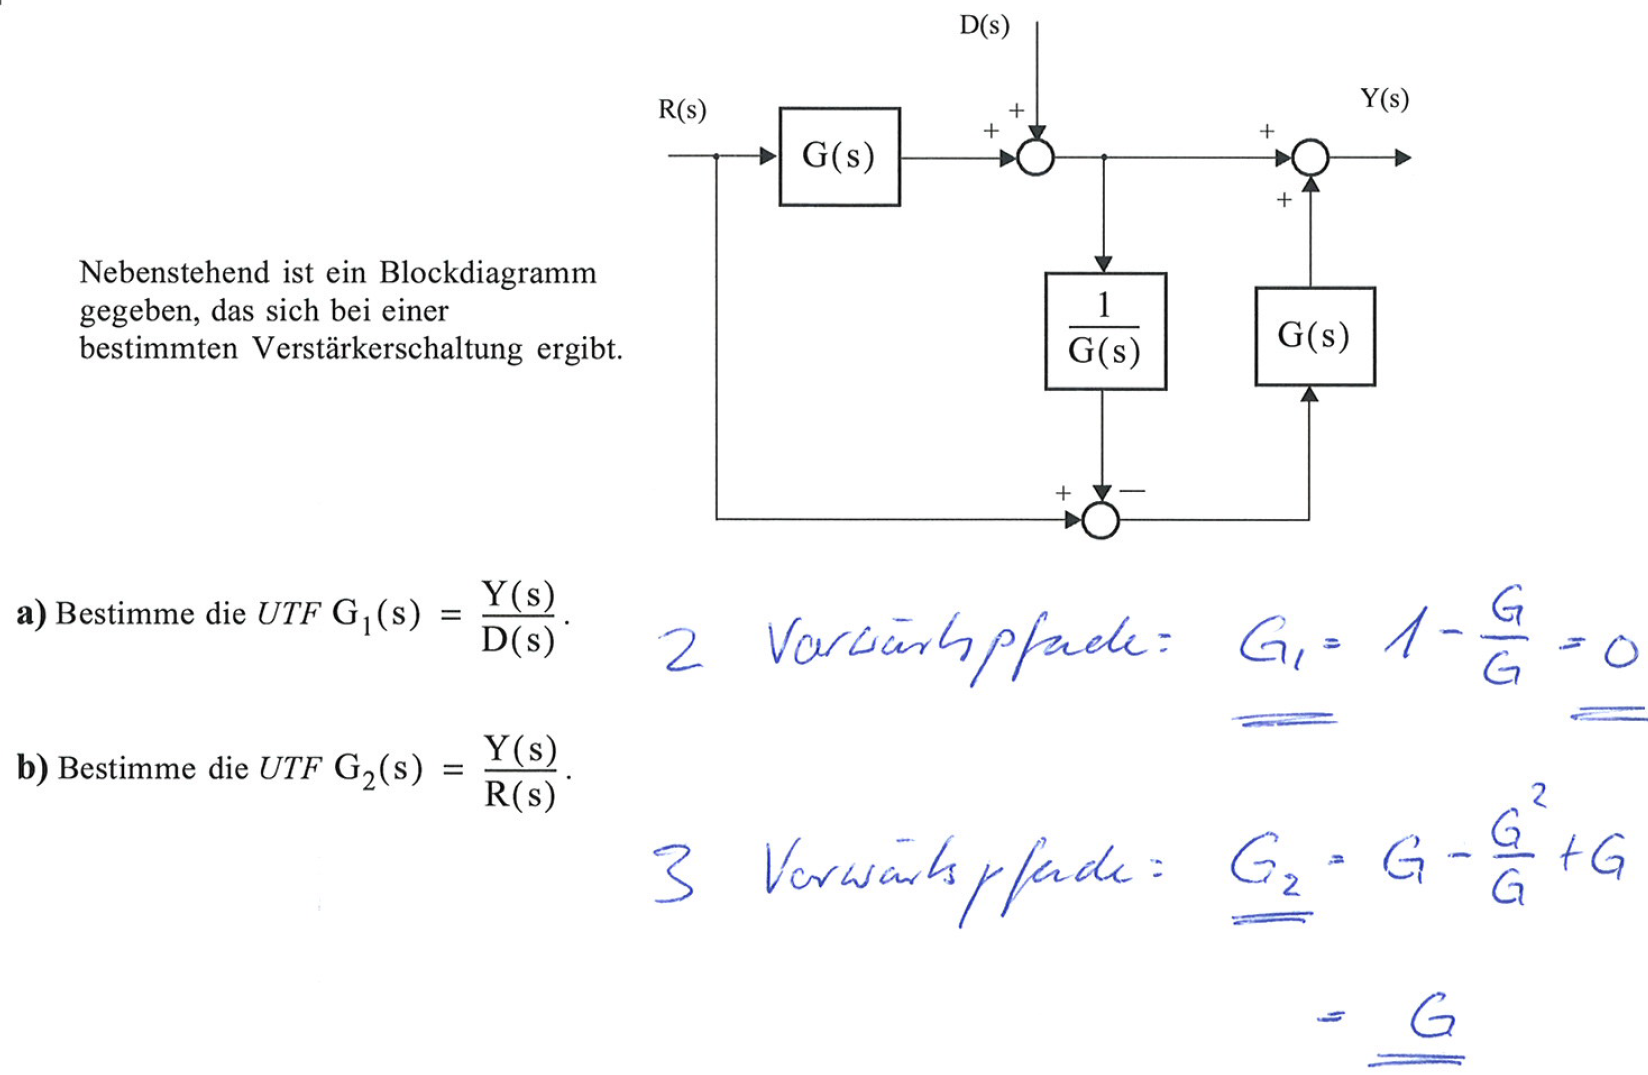
\includegraphics[width=9cm]{./images/beispiele/beispiel6.png}
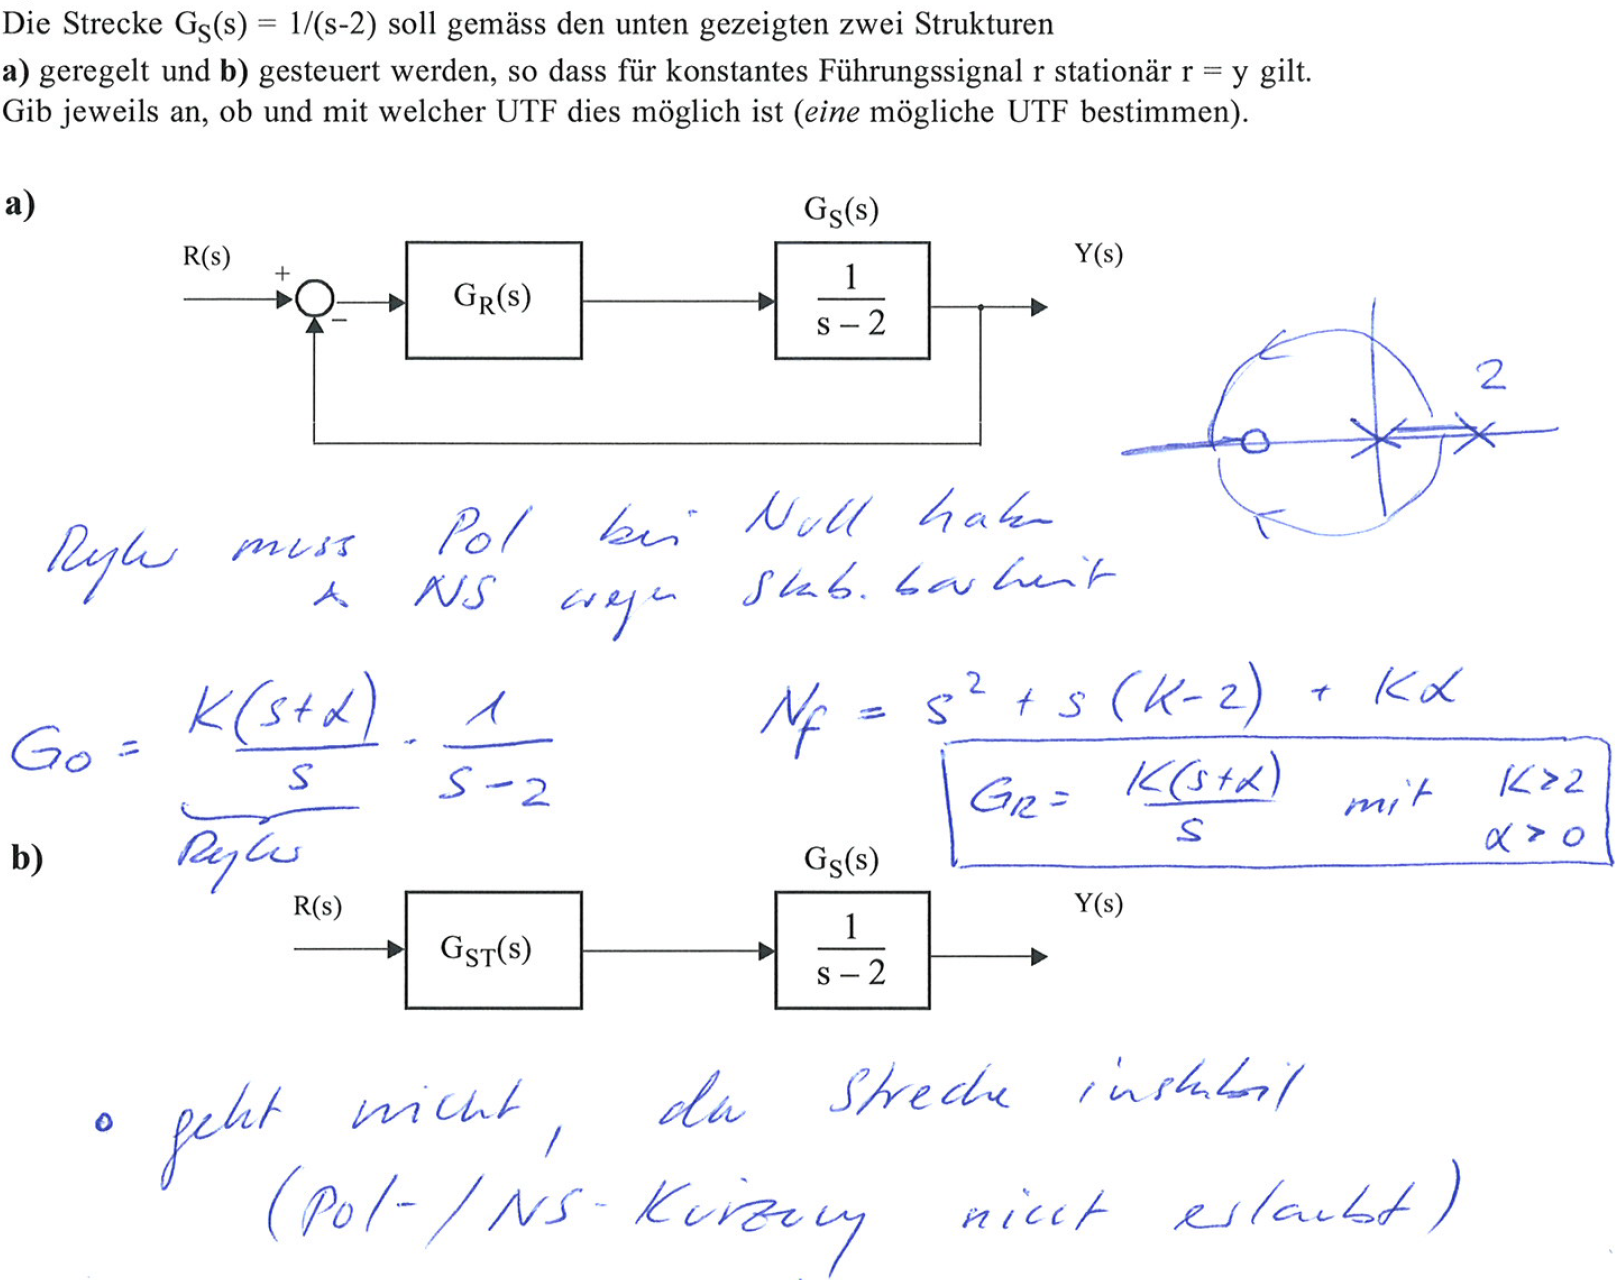
\includegraphics[width=9cm]{./images/beispiele/beispiel7.png}
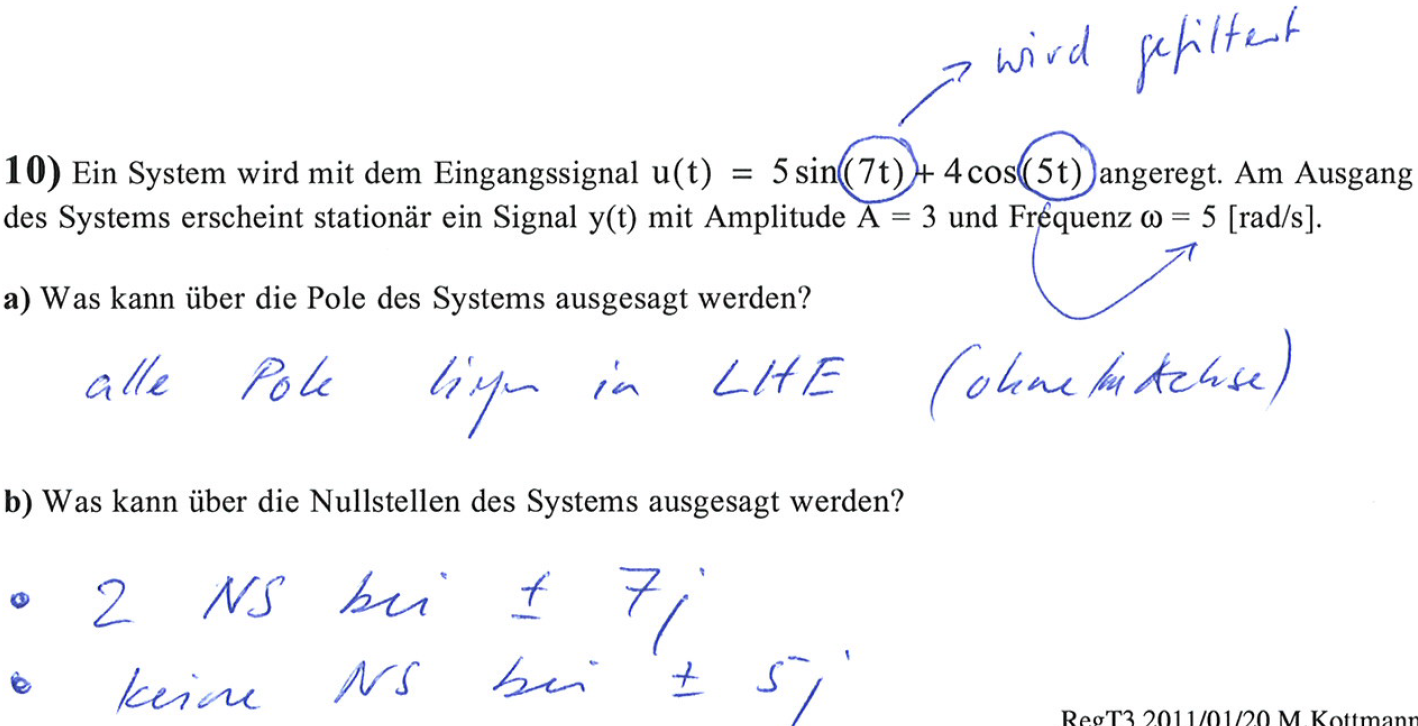
\includegraphics[width=9cm]{./images/beispiele/beispiel8.png}
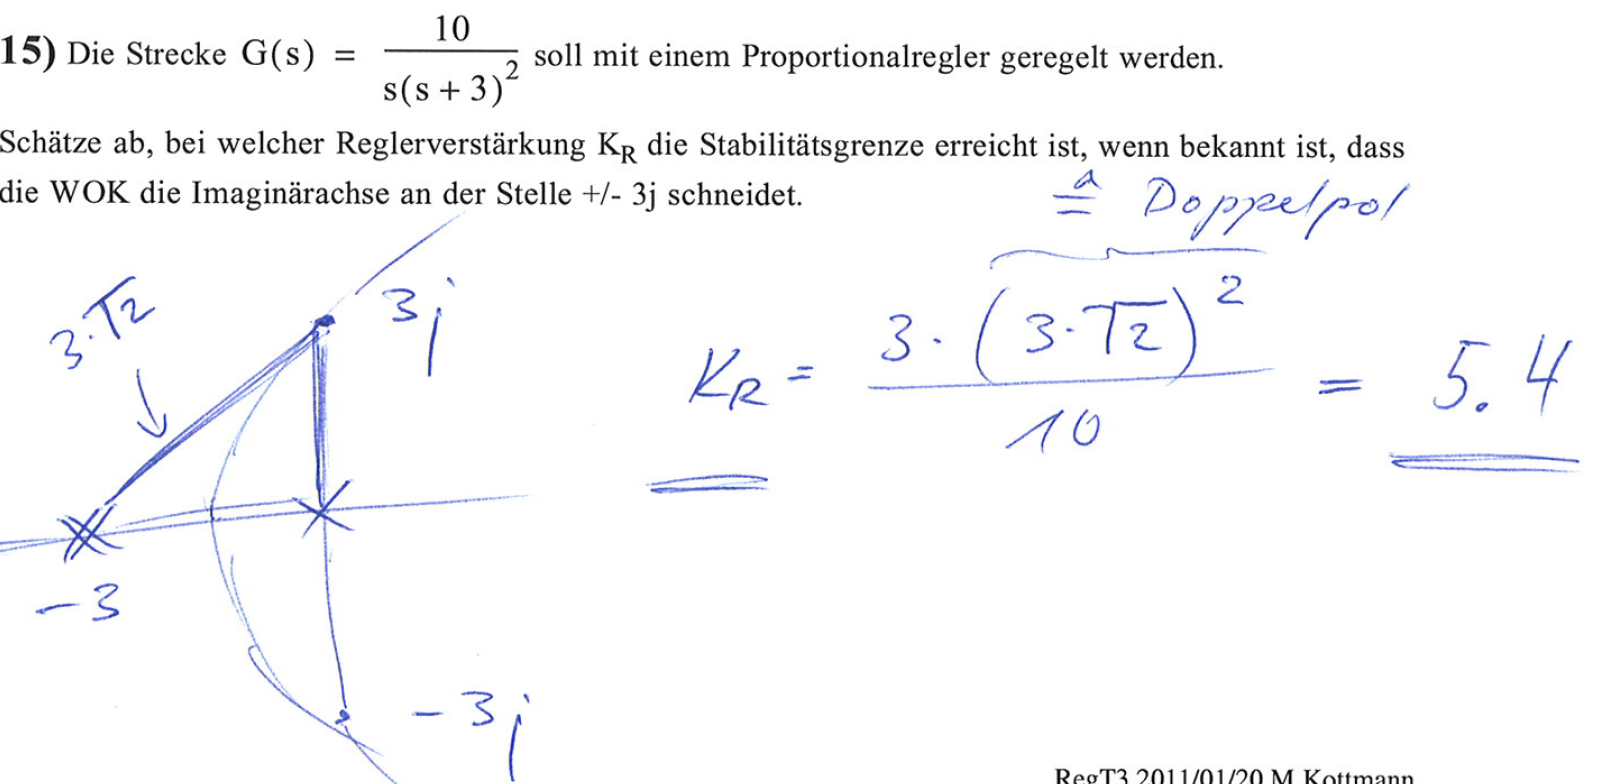
\includegraphics[width=9cm]{./images/beispiele/beispiel9.png}
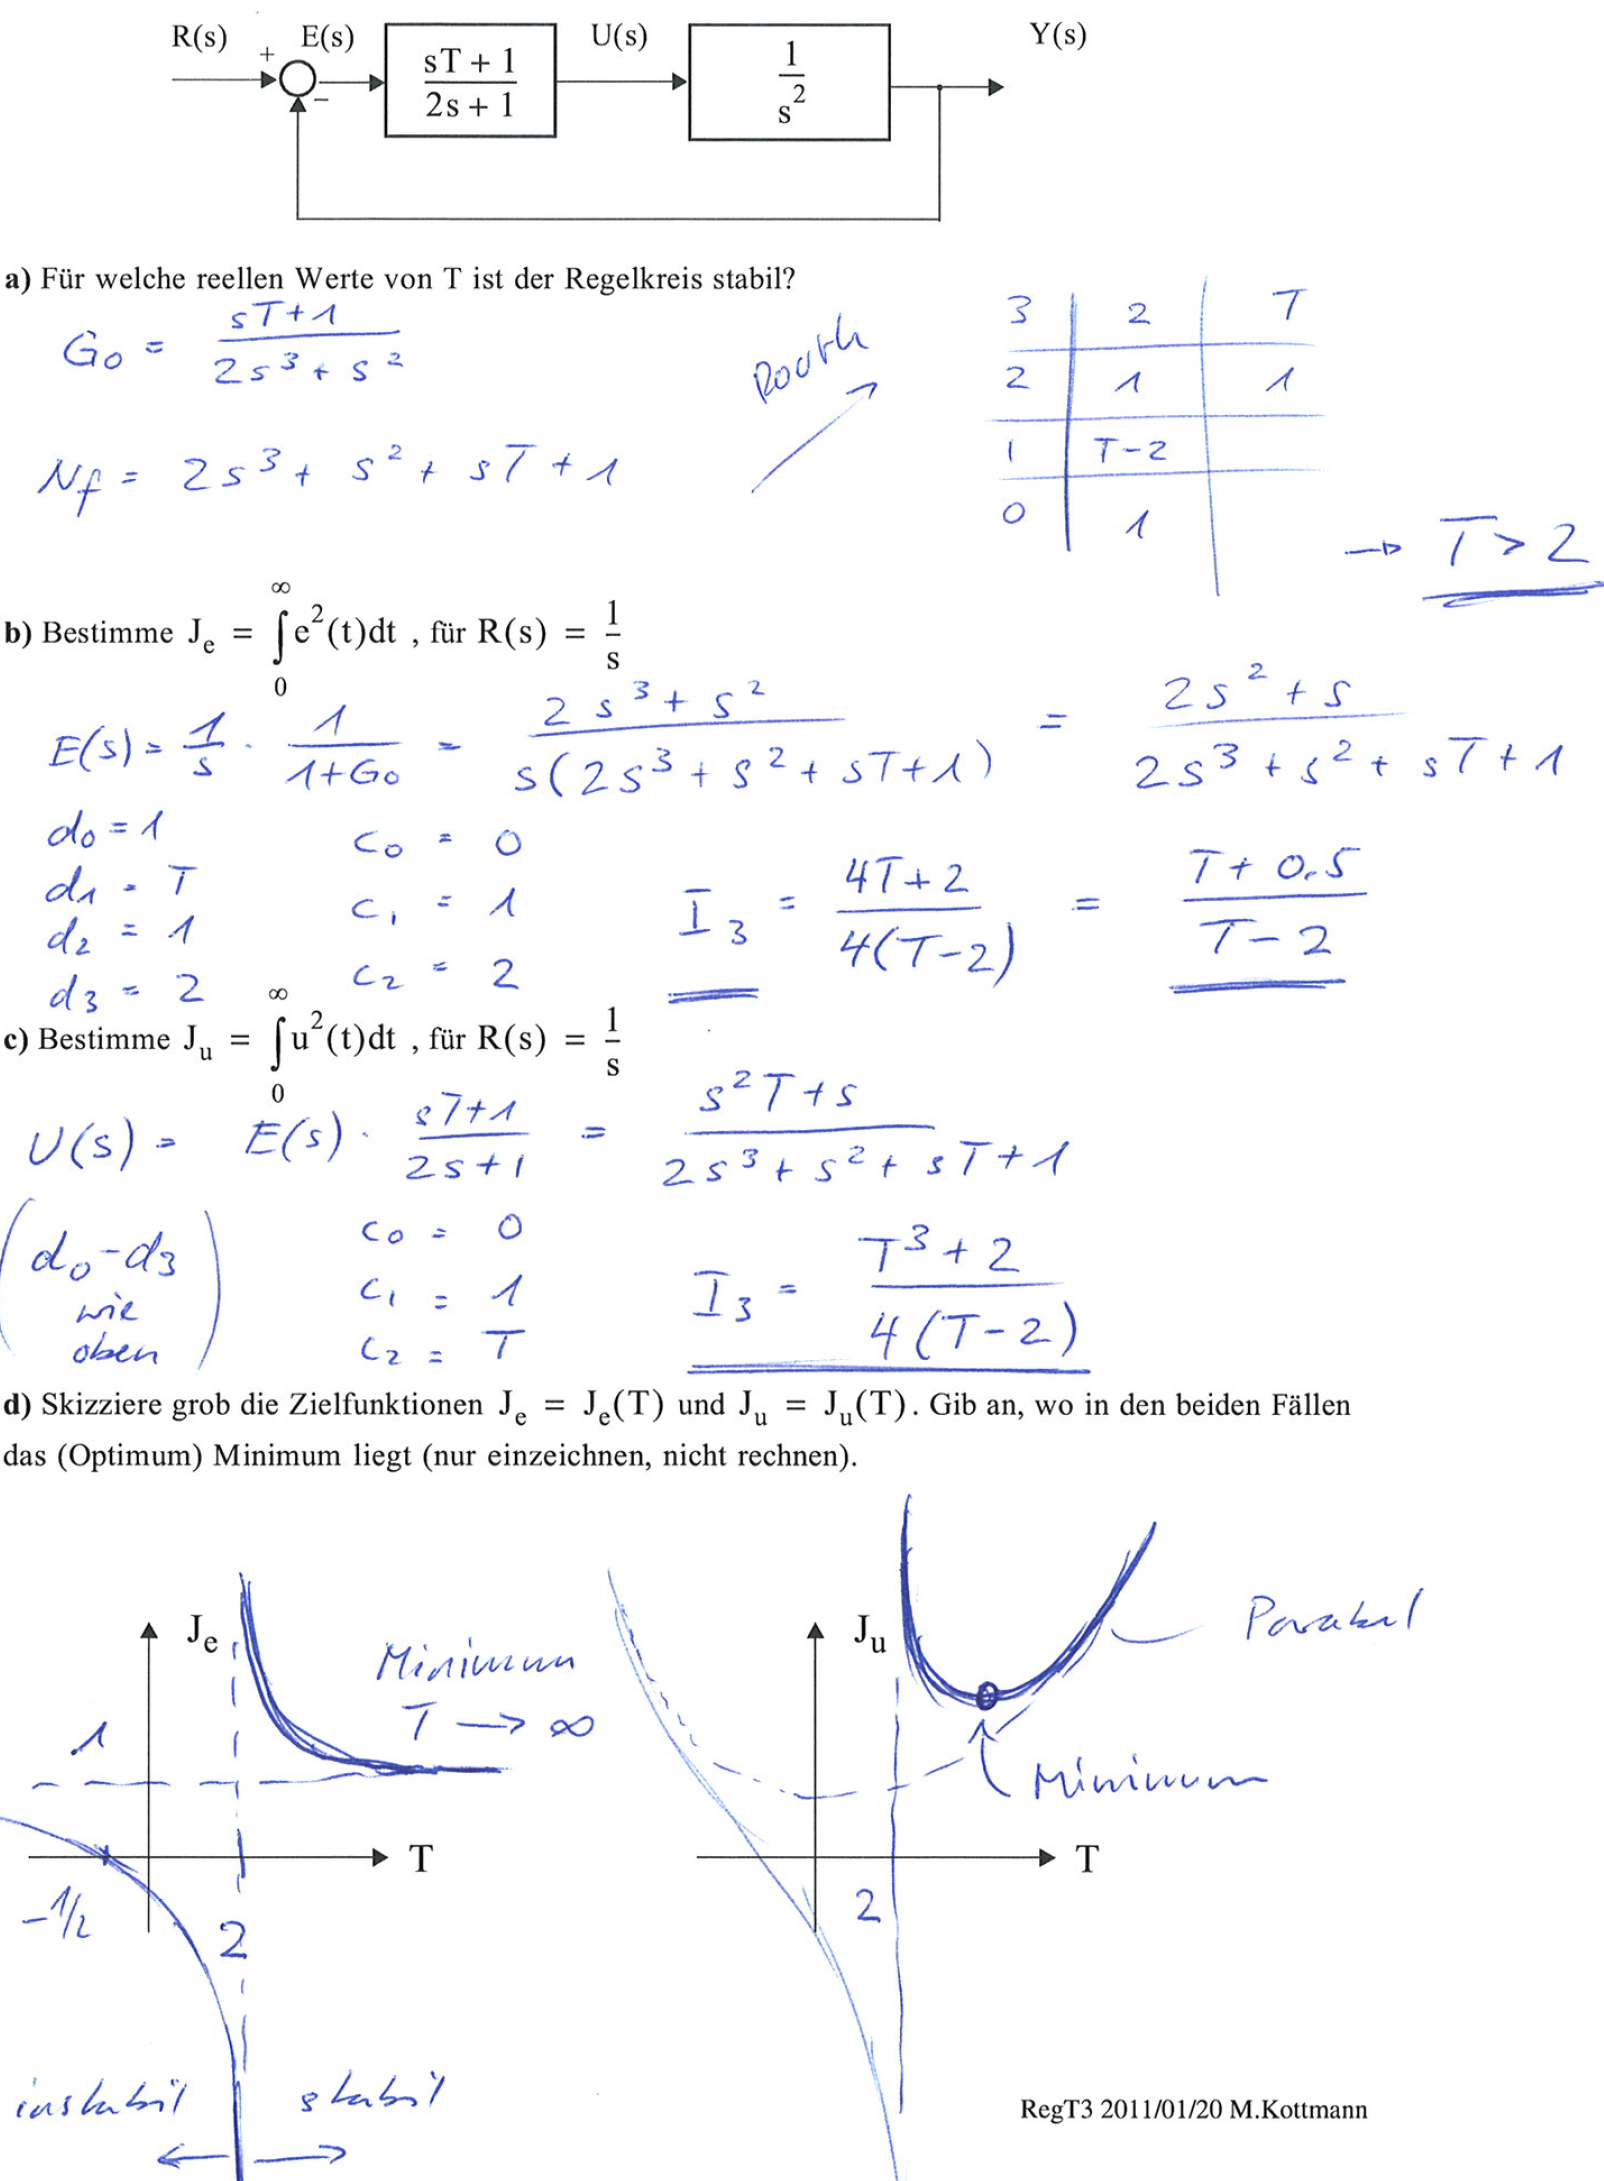
\includegraphics[width=9cm]{./images/beispiele/beispiel10.png}
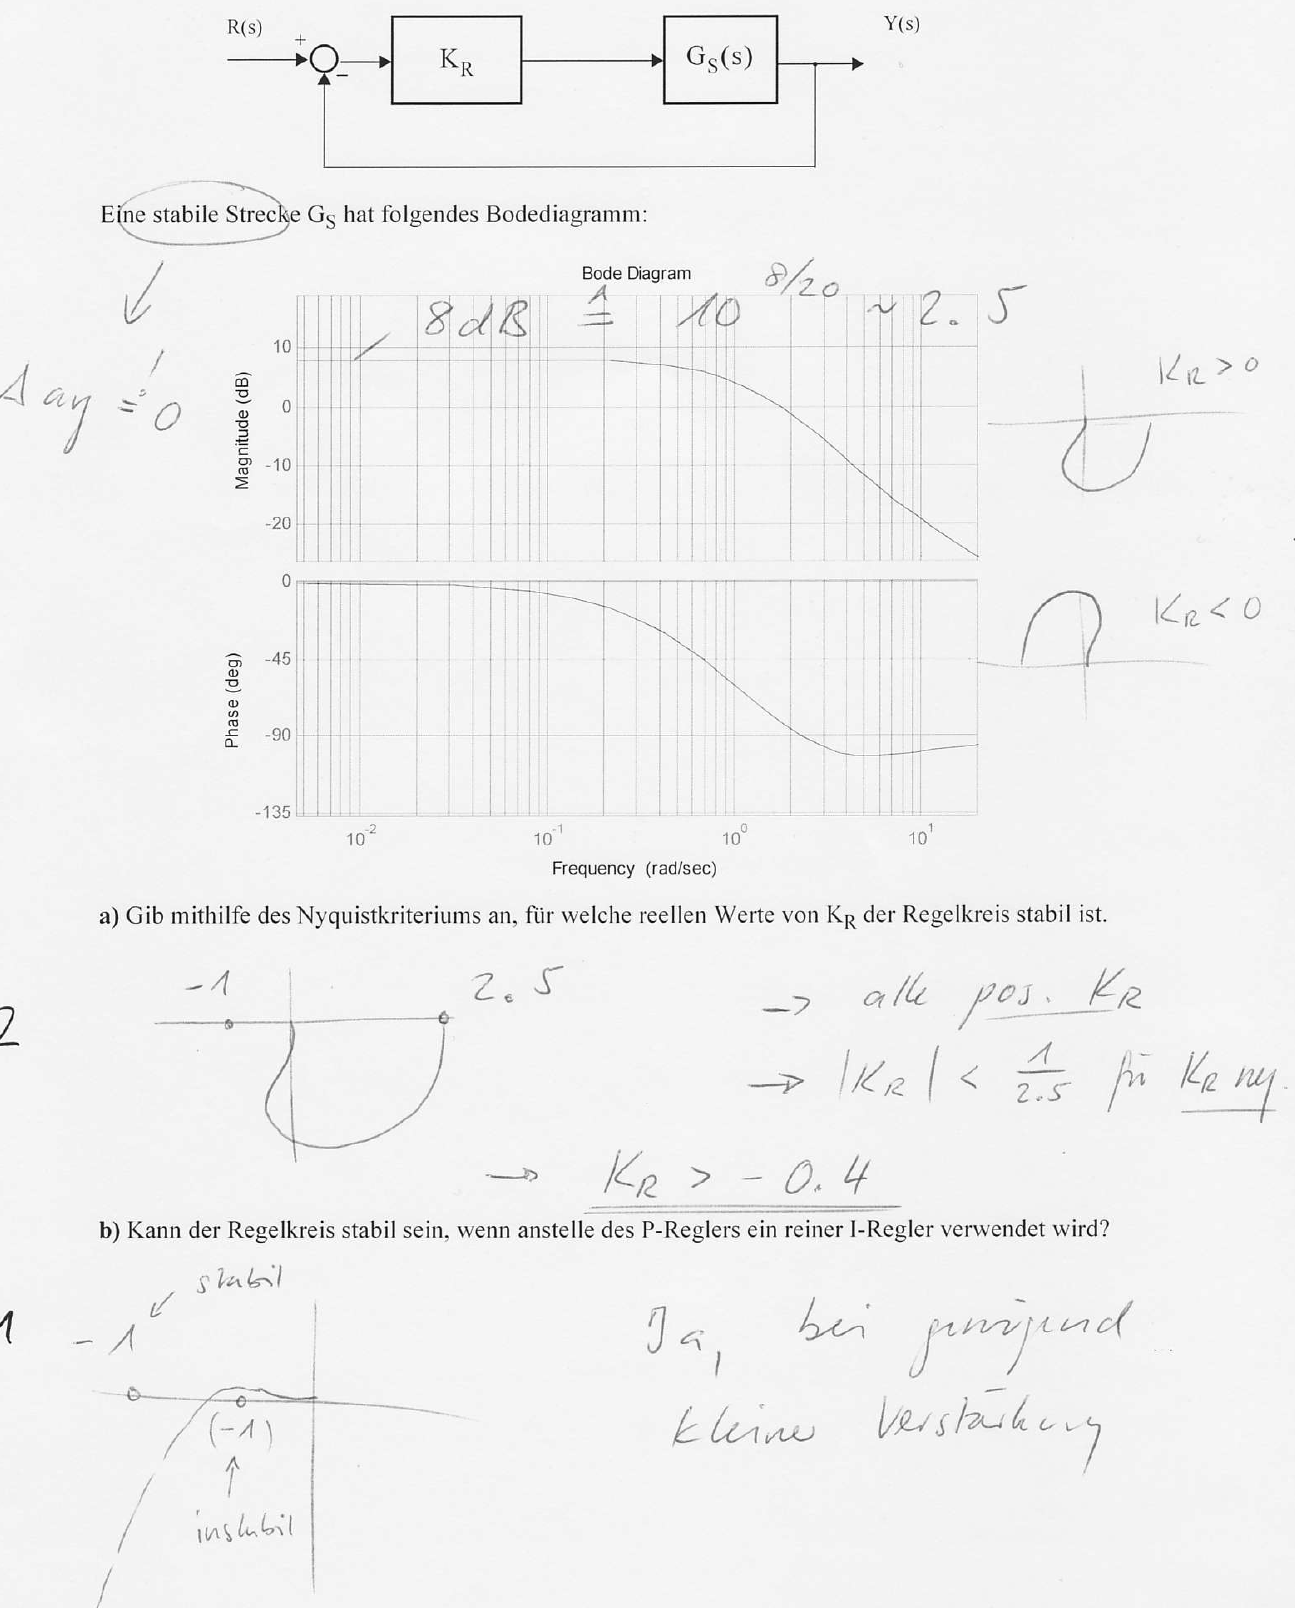
\includegraphics[width=9cm]{./images/beispiele/beispiel11.png}
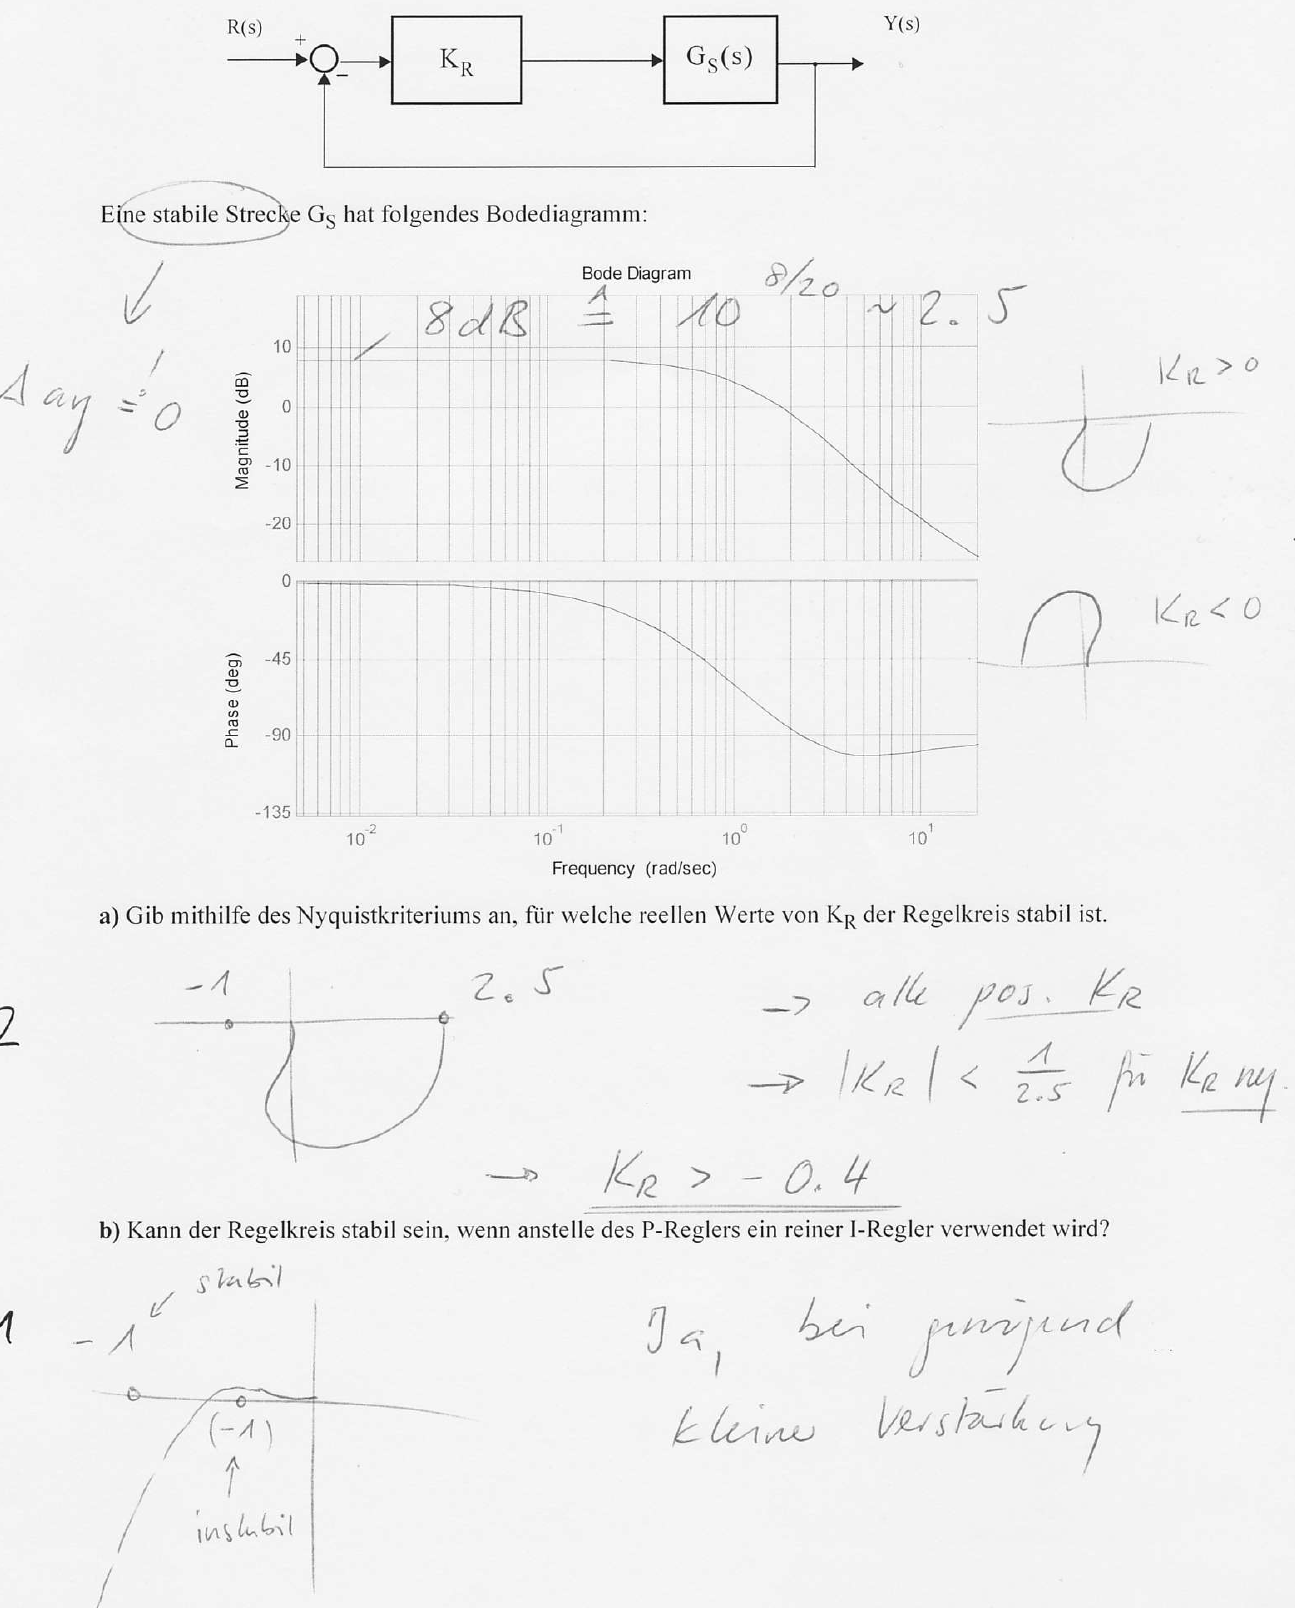
\includegraphics[width=9cm]{./images/beispiele/beispiel12.png}
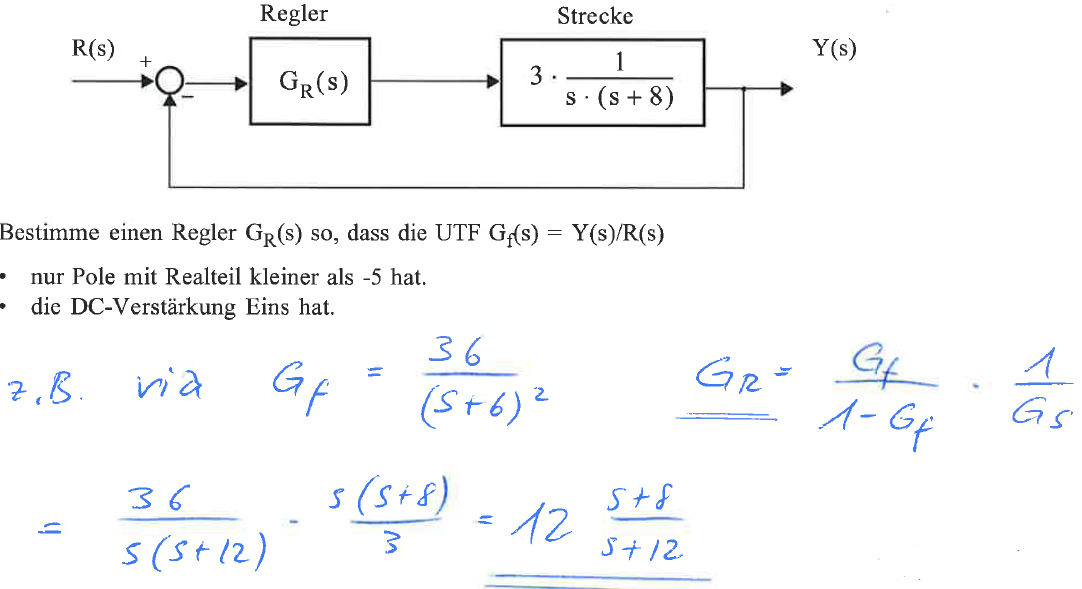
\includegraphics[width=9cm]{./images/beispiele/beispiel13.png}
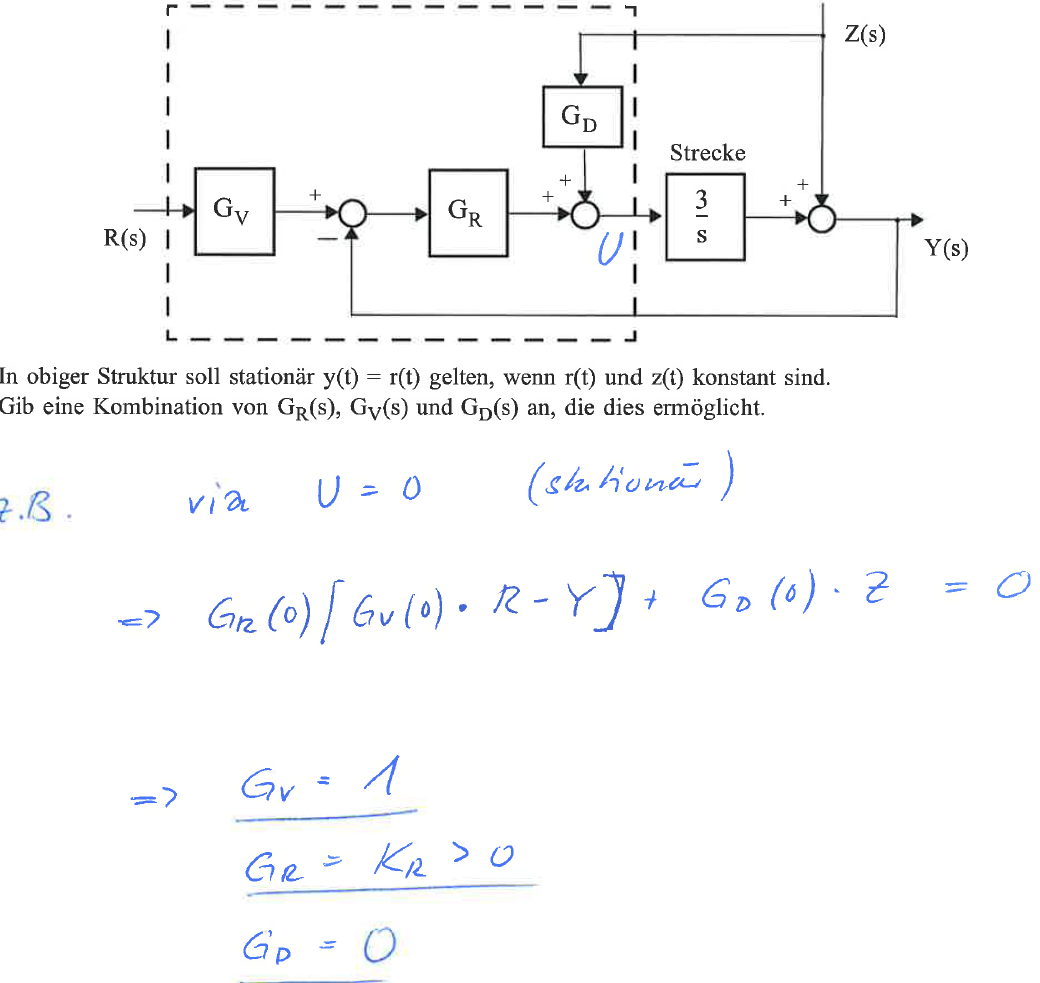
\includegraphics[width=9cm]{./images/beispiele/beispiel14.png}
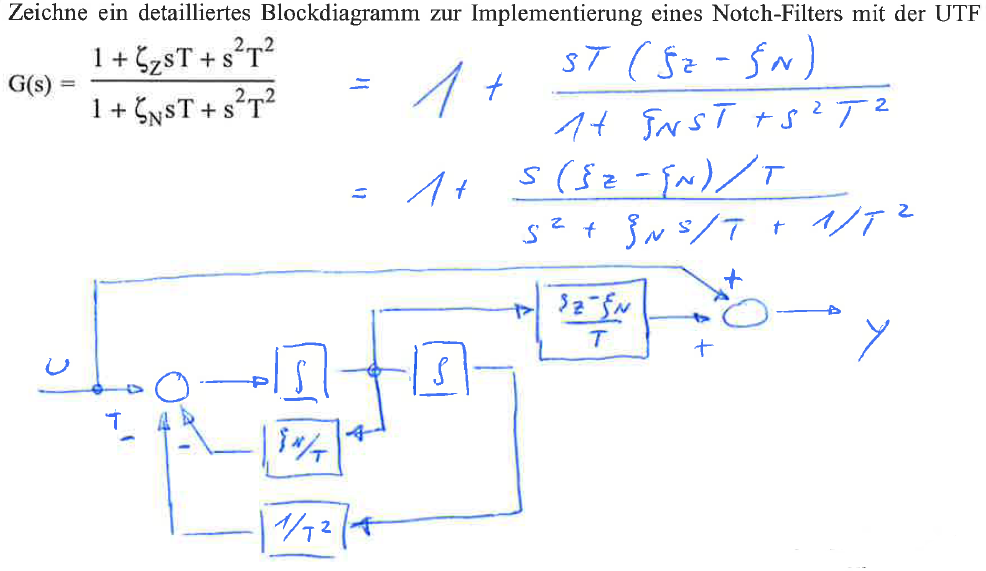
\includegraphics[width=9cm]{./images/beispiele/beispiel15.png}
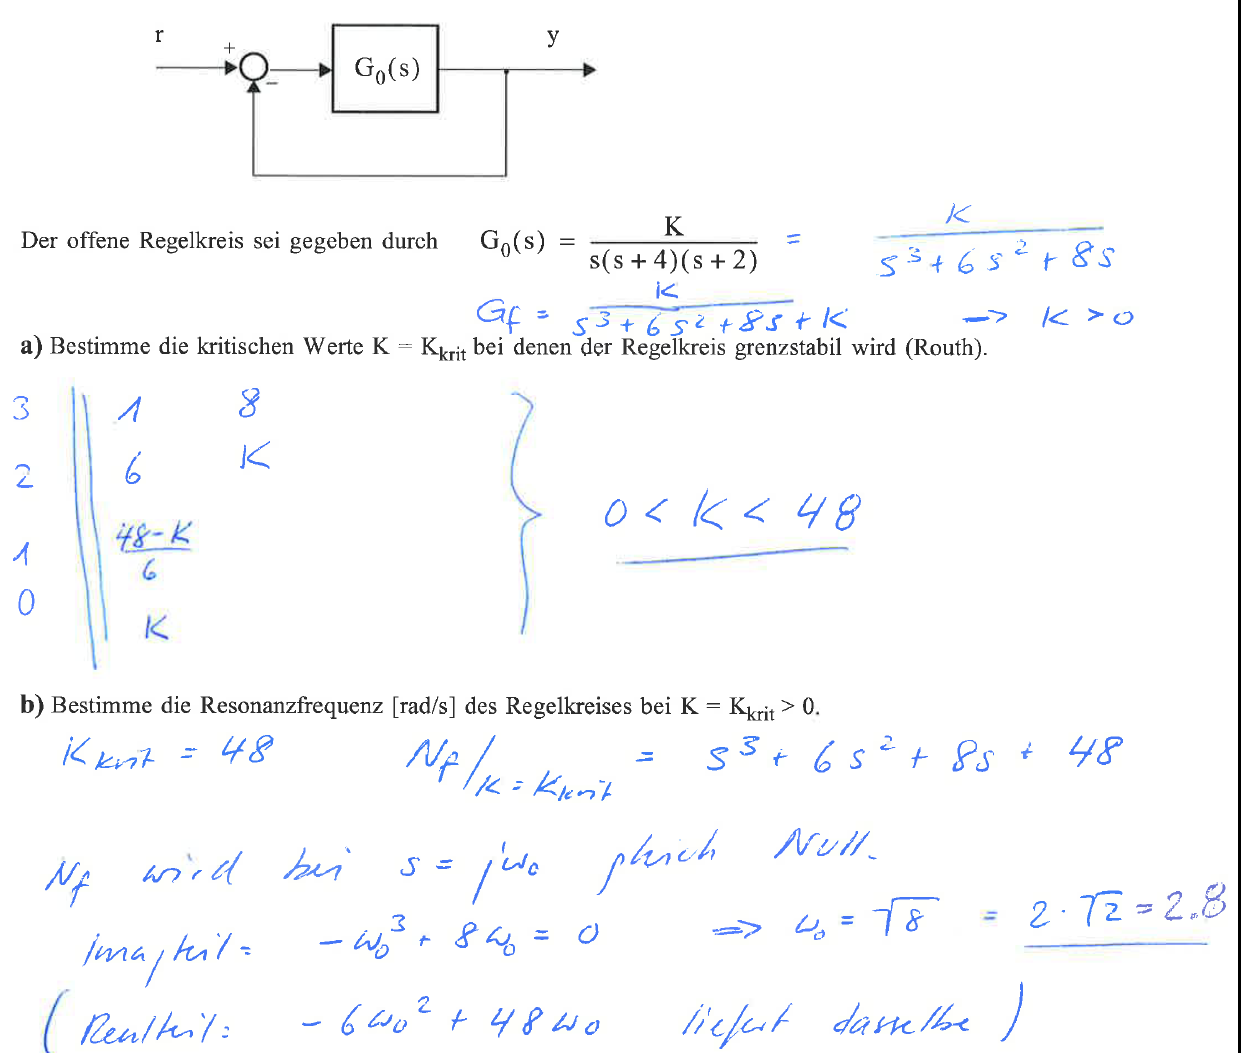
\includegraphics[width=9cm]{./images/beispiele/beispiel16.png}
\end{multicols}

